%% FullCourse_10Lecs -- Lecture 3, Topic 3.4: Specialized Architectures + Curve Fitting + Lab
%% Source: ./archive_pre_split/Lec03_ML_for_Macro.tex (sections 7-9 + summary)
%% Pass B: layer in refinements from
%%         ../../MiniCourse_8hr/Slides/Module1_ML_Foundations/M1_T4_Specialized_Networks.tex

%% Shared preamble for the FullCourse_10Lecs topic decks.
%%
%% Each topic .tex \input's this file, then defines its own \title, \date
%% override (if any), \graphicspath, and \begin{document}.
%%
%% Reconstructed verbatim from the inlined copy preserved in
%% Lec10_Case_Studies/Lec10_T8_Case6_DeepRamsey.tex (lines 23-190), which is
%% explicitly annotated there as "from ../shared_preamble.tex, copied verbatim".
%% Base preamble matches MiniCourse_8hr/Slides/shared_preamble.tex; this version
%% additionally provides \sectiondivider, the conceptbox/cautionbox/examplebox/
%% takeawaybox tcolorboxes, and \compacttables used across the split decks.

\documentclass[10pt,english,aspectratio=169]{beamer}

\usepackage{ae,aecompl}
\usepackage[T1]{fontenc}
\usepackage{textcomp}
\usepackage[utf8]{inputenc}
\usepackage{babel}
\usepackage{datetime2}

\setcounter{secnumdepth}{3}
\setcounter{tocdepth}{3}

\usepackage{amsmath, amssymb, amsthm, graphicx}
\usepackage{booktabs, multirow}
\usepackage{tikz}
\usepackage{pgfplots}
\pgfplotsset{compat=1.16}
\usepackage[most]{tcolorbox}
\tcbuselibrary{skins, breakable, theorems}
\usepackage{listings}
\usepackage{xcolor}

\lstset{
  basicstyle=\ttfamily\small,
  keywordstyle=\color{blue!80!black}\bfseries,
  commentstyle=\color{green!50!black}\itshape,
  stringstyle=\color{orange!80!black},
  backgroundcolor=\color{gray!8},
  frame=single,
  rulecolor=\color{gray!40},
  breaklines=true,
  showstringspaces=false,
  numbers=none,
}

\lstdefinestyle{pythonstyle}{
    language=Python,
    basicstyle=\ttfamily\footnotesize,
    keywordstyle=\color{blue!80!black}\bfseries,
    commentstyle=\color{green!50!black}\itshape,
    stringstyle=\color{orange!80!black},
    frame=single,
    breaklines=true,
    showstringspaces=false,
    numbers=left,
    numbersep=5pt,
    numberstyle=\tiny\color{gray},
    backgroundcolor=\color{gray!8},
    rulecolor=\color{gray!40}
}

\ifx\hypersetup\undefined
  \AtBeginDocument{%
    \hypersetup{bookmarks=false,breaklinks=true,pdfborder={0 0 0},colorlinks=true,
      linkcolor=DarkText,urlcolor=RedTitle}%
  }
\else
  \hypersetup{bookmarks=false,breaklinks=true,pdfborder={0 0 0},colorlinks=true,
    linkcolor=DarkText,urlcolor=RedTitle}%
\fi

\makeatletter
\newcommand\makebeamertitle{%
  \begin{frame}[plain]
    \vspace*{1.0cm}
    \centering
    {\usebeamerfont{title}\usebeamercolor[fg]{title}\inserttitle\par}
    \vspace{1.0cm}
    {\usebeamerfont{author}\usebeamercolor[fg]{author}\insertauthor\par}
    \vspace{0.2cm}
    {\usebeamerfont{date}\usebeamercolor[fg]{date}\insertdate\par}
  \end{frame}}%
\AtBeginDocument{%
  \let\origtableofcontents=\tableofcontents
  \def\tableofcontents{\@ifnextchar[{\origtableofcontents}{\gobbletableofcontents}}
  \def\gobbletableofcontents#1{\origtableofcontents}%
}

\usetheme{metropolis}
\usefonttheme{professionalfonts}

\definecolor{LightGray}{RGB}{230,230,230}
\definecolor{RedTitle}{RGB}{0,0,200}
\definecolor{VeryLightGray}{RGB}{245,245,245}
\definecolor{DarkText}{RGB}{0,0,0}

\setbeamercolor{background canvas}{bg=white}
\setbeamercolor{title}{fg=RedTitle}
\setbeamercolor{author}{fg=DarkText}
\setbeamercolor{date}{fg=DarkText}
\setbeamercolor{frametitle}{bg=VeryLightGray,fg=DarkText}
\setbeamercolor{normal text}{fg=DarkText}
\setbeamerfont{title}{size=\large}

\setbeamersize{text margin left=5mm, text margin right=5mm}
\addtobeamertemplate{frametitle}{}{\vspace{-0.5em}}
\newcommand{\reducevspace}{\vspace{-0.5cm}}

% Shared section divider and box styles for split topic decks.
\newcommand{\sectiondivider}[2]{%
\begin{frame}[plain,noframenumbering]
\begin{center}
\vfill
{\Large\textbf{#1}\par}
\vspace{0.35cm}
{\normalsize #2\par}
\vfill
\end{center}
\end{frame}
}

\newtcolorbox{conceptbox}[1][]{
  colback=blue!3,
  colframe=RedTitle!55,
  boxrule=0.35mm,
  arc=1mm,
  left=2mm,
  right=2mm,
  top=1mm,
  bottom=1mm,
  #1
}
\newtcolorbox{cautionbox}[1][]{
  colback=red!3,
  colframe=red!50!black,
  boxrule=0.35mm,
  arc=1mm,
  left=2mm,
  right=2mm,
  top=1mm,
  bottom=1mm,
  #1
}
\newtcolorbox{examplebox}[1][]{
  colback=green!3,
  colframe=green!45!black,
  boxrule=0.35mm,
  arc=1mm,
  left=2mm,
  right=2mm,
  top=1mm,
  bottom=1mm,
  #1
}
\newtcolorbox{takeawaybox}[1][]{
  colback=VeryLightGray,
  colframe=RedTitle!55,
  boxrule=0.35mm,
  arc=1mm,
  left=2mm,
  right=2mm,
  top=1mm,
  bottom=1mm,
  #1
}
\newcommand{\compacttables}{\renewcommand{\arraystretch}{1.15}}

\setbeamertemplate{navigation symbols}{}
\setbeamertemplate{footline}{%
  \hfill%
  \usebeamercolor[fg]{page number in head/foot}%
  \usebeamerfont{page number in head/foot}%
  \insertframenumber\,/\,\inserttotalframenumber\kern1em\vskip2pt%
}

\makeatother

\author{Zhigang Feng}
% "date with time": compile timestamp so each build is identifiable.
\date{\today\ \DTMcurrenttime}

\usepackage{colortbl}

\graphicspath{{./pic/}{../../MiniCourse_8hr/Slides/Module1_ML_Foundations/pic/}{../}}

% Suppress the redundant auto-generated metropolis section page; the
% \sectiondivider frames below are the dividers we keep.
\metroset{sectionpage=none}
\usetikzlibrary{positioning,arrows.meta,shapes,calc}
%% Lec03 shared MAP slide: "one map, four acts" recurring diagram.
%% Input this file AFTER ../shared_preamble.tex (needs RedTitle, VeryLightGray,
%% DarkText) and AFTER \usetikzlibrary{positioning,arrows.meta,shapes,calc}.
%% Call \LecThreeMap{k} inside a frame, where k in {1,2,3,4} highlights the
%% current act ("you are here") and k = 0 renders the closing reprise with all
%% four acts checked green (used by T4's closing frame).
%% Filename deliberately does NOT match the build glob Lec*_T*.tex, so the build
%% script never tries to compile it standalone.
%%
%% The four acts are the lecture's story: WHY -> BUILD -> TRAIN -> SHAPE, i.e.
%% the case for ML in economics, the network as an object (architecture + UAT),
%% the learning machinery (backprop + SGD + regularization + double descent),
%% and economics-aware architectures with the hands-on lab.

\newcommand{\LecThreeMap}[1]{%
% Precompute per-box style selectors; TikZ option lists are comma-split before
% TeX conditionals run, so \ifnum must not sit inside a [...] options list.
\ifnum#1=0
  \tikzset{lmapa/.style={lmapdone}, lmapb/.style={lmapdone},
           lmapc/.style={lmapdone}, lmapd/.style={lmapdone}}%
\else
  \tikzset{lmapa/.style={}, lmapb/.style={}, lmapc/.style={}, lmapd/.style={}}%
  \ifnum#1=1 \tikzset{lmapa/.style={lmapcur}}\fi
  \ifnum#1=2 \tikzset{lmapb/.style={lmapcur}}\fi
  \ifnum#1=3 \tikzset{lmapc/.style={lmapcur}}\fi
  \ifnum#1=4 \tikzset{lmapd/.style={lmapcur}}\fi
\fi
\begin{center}
\begin{tikzpicture}[
    act/.style={rectangle, rounded corners, draw=black!60, fill=VeryLightGray,
        minimum width=3.0cm, minimum height=0.95cm, text width=2.9cm,
        align=center, font=\small, text=DarkText},
    lmapcur/.style={draw=RedTitle, very thick, fill=orange!20},
    lmapdone/.style={draw=green!45!black, thick, fill=green!10},
    q/.style={font=\tiny\itshape, text width=3.0cm, align=center, text=black!70},
    barlab/.style={font=\tiny\bfseries, text=black!65},
    sat/.style={rectangle, rounded corners, draw=black!45, dashed, fill=white,
        text width=5.2cm, align=center, font=\tiny, text=black!70,
        minimum height=0.5cm},
    arr/.style={-{Stealth[length=2.2mm]}, thick, gray!60}
]
    % --- four act boxes ---
    \node[act, lmapa] (a1) at (0,0)
        {\textbf{3.1\ \ WHY}\\[1pt] \tiny the case for ML in econ};
    \node[act, lmapb] (a2) at (3.6,0)
        {\textbf{3.2\ \ BUILD}\\[1pt] \tiny neurons $\cdot$ activations $\cdot$ UAT};
    \node[act, lmapc] (a3) at (7.2,0)
        {\textbf{3.3\ \ TRAIN}\\[1pt] \tiny backprop $\cdot$ SGD $\cdot$ dbl.\ descent};
    \node[act, lmapd] (a4) at (10.8,0)
        {\textbf{3.4\ \ SHAPE}\\[1pt] \tiny ICNN $\cdot$ monotone $\cdot$ lab};
    \draw[arr] (a1) -- (a2);
    \draw[arr] (a2) -- (a3);
    \draw[arr] (a3) -- (a4);
    % --- the student question each act answers ---
    \node[q] at (0,-0.95)    {why should an economist\\ care about ML?};
    \node[q] at (3.6,-0.95)  {what is a neural network,\\ and why does it work?};
    \node[q] at (7.2,-0.95)  {how does it learn ---\\ and why not overfit?};
    \node[q] at (10.8,-0.95) {how do I build economics\\ in --- and run it myself?};
    % --- "you are here" marker above the current act ---
    \ifnum#1=1 \node[font=\scriptsize\bfseries, text=RedTitle] at (0,0.98)
        {you are here\ $\blacktriangledown$};\fi
    \ifnum#1=2 \node[font=\scriptsize\bfseries, text=RedTitle] at (3.6,0.98)
        {you are here\ $\blacktriangledown$};\fi
    \ifnum#1=3 \node[font=\scriptsize\bfseries, text=RedTitle] at (7.2,0.98)
        {you are here\ $\blacktriangledown$};\fi
    \ifnum#1=4 \node[font=\scriptsize\bfseries, text=RedTitle] at (10.8,0.98)
        {you are here\ $\blacktriangledown$};\fi
    \ifnum#1=0 \node[font=\scriptsize\bfseries, text=green!45!black] at (5.4,0.98)
        {all four acts complete};\fi
    % --- bottom band: the ML pipeline (the technical spine of the lecture) ---
    \fill[blue!10]   (-1.55,-1.72) rectangle (5.15,-1.40);
    \fill[green!12]  (5.65,-1.72)  rectangle (8.75,-1.40);
    \fill[orange!16] (9.25,-1.72)  rectangle (12.35,-1.40);
    \node[barlab] at (1.8,-1.56)  {REPRESENT\ (UAT $\cdot$ Barron)};
    \node[barlab] at (7.2,-1.56)  {OPTIMIZE\ (loss $\cdot$ gradient)};
    \node[barlab] at (10.8,-1.56) {GENERALIZE $+$ CONSTRAIN};
    % --- dashed satellites: where this lecture sits in the course flow ---
    \node[sat] at (1.5,-2.42)
        {\textit{upstream:} Lec01--02 --- AI as cognitive capital; deep learning as the engine of the predictive stack};
    \node[sat] at (9.3,-2.42)
        {\textit{downstream:} Lec04--06 --- these networks become Bellman/Euler solvers for dynamic macro models};
\end{tikzpicture}
\end{center}
}


\title[AI for Econ Research]{AI for Economic Research: Dynamic Models, Language, and Agents\\
Lecture 3.4: Specialized Architectures \& Curve-Fitting Case}

\begin{document}

\makebeamertitle

%=============================================================================
\begin{frame}{Lecture 3 in One Map}
\textbf{One lecture, four decks, one goal: make neural networks a working tool for economists --- why they matter, what they are, how they learn, and how to make them respect economics.}

\LecThreeMap{4}

\vspace{0.05cm}
\footnotesize\textit{\textbf{Act 3.4 (here)} closes the loop: ICNN and monotone networks hard-wire economic shape restrictions, a curve-fitting race (polynomial vs.\ Chebyshev vs.\ DNN) makes it concrete, and the lab walkthrough (\texttt{Lec03\_Lab\_ML\_Basics}) hands you the code.}
\end{frame}

%=============================================================================
\section{Specialized Architectures}

\sectiondivider{Specialized Architectures}{ICNN and monotone networks: hard-wiring economic shape restrictions}

% FullCourse Pass B addition: ports MiniCourse M1_T4 motivation framing.
\begin{frame}{Why Standard FFNNs Fall Short in Quant Macro}
\begin{itemize}
  \item \textbf{Nested ``Russian Doll'' structure}: Quantitative macro models involve \emph{multiple} nested optimization problems.
  \medskip
  \item \textbf{Typical hierarchy}:
    \begin{enumerate}
      \item \textbf{Outer Loop}: Market clearing / calibration (solve for prices $p^*$)
      \item \textbf{Middle Loop}: Value function iteration (solve Bellman equations)
      \item \textbf{Inner Loop}: Agent optimization (choose $c, \ell, k'$ given state and prices)
    \end{enumerate}
  \medskip
  \item \textbf{Problem}: Approximating value functions or costs with generic FFNNs turns the \emph{inner} problem into a non-convex optimization
    \begin{itemize}
      \item Multiple local optima and unstable outer iterations
      \item Economic misspecification (e.g., upward-sloping demand, non-concave value functions)
    \end{itemize}
\end{itemize}
\end{frame}

% FullCourse Pass B addition: economic-structure $\to$ architecture mapping table.
\begin{frame}{Idea: Inject Economic Structure into the Network}
\textbf{Key idea}: Design architectures that \emph{respect} economic shape restrictions \emph{by construction}.

\vspace{0.3cm}
\centering
\renewcommand{\arraystretch}{1.4}
\begin{tabular}{l | l | l}
\textbf{Property} & \textbf{Mathematical Gain} & \textbf{Economic Payoff} \\
\hline
Convexity / Concavity & Unique global optimum & Stable policy rules / VFI \\
\hline
Monotonicity & Invertible mappings & Well-behaved supply/demand \\
\hline
Homogeneity & $f(\lambda x) = \lambda f(x)$ & Consistency with balanced growth \\
\end{tabular}

\vspace{0.3cm}
\raggedright
\begin{itemize}
  \item This turns the neural net from a \textbf{black box} into a \textbf{glass box}: flexible enough to fit data, but disciplined by theory.
\end{itemize}
\end{frame}

\begin{frame}{Convolution: Sliding a Small Filter Over the Input}
\textbf{Three objects} (first conv layer, classifying a handwritten digit):
\begin{itemize}
\item \textbf{Input $X$} --- the image: a grid of numbers (e.g.\ a $28\times28$ intensity map); in deeper layers, the previous layer's feature map.
\item \textbf{Filter / kernel $W$} --- a \emph{small} grid of \textbf{learned} weights (e.g.\ $3\times3$): a ``pattern template.''
\item \textbf{Output $Y$} --- the \textbf{feature map}: one number per location, scoring how strongly $W$'s pattern appears there.
\end{itemize}

\smallskip
\textbf{What convolution does:} slide $W$ across $X$; at each spot overlay the filter, multiply overlapping cells, and add them (a local weighted dot product):
\[
\underbrace{Y(i,j)}_{\text{output}} \;=\; \sum_m \sum_n \underbrace{X(i-m,\,j-n)}_{\text{input patch}}\, \underbrace{W(m,n)}_{\text{filter weight}}
\]
$Y(i,j)$ is \textbf{large} where the local patch of $X$ \emph{looks like} the pattern in $W$ (an edge, a curve, a stroke).

\smallskip
\textbf{Weight sharing:} the same tiny $W$ is reused everywhere --- it finds its feature \emph{wherever} it occurs (translation equivariance), with far fewer parameters than a dense layer.
\end{frame}

\begin{frame}{Pooling --- and Why a CNN Is a ``Learned Manifold Map''}
\textbf{Pooling: shrink and summarize.} Replace each small window $R$ of the feature map with one summary value; \textbf{max-pooling} keeps the strongest response:
\[
\text{MaxPool}(i,j) = \max_{(m,n)\in R} X(m,n)
\]
\begin{itemize}
\item \textbf{Downsamples} (less compute) and adds \textbf{translation invariance} --- ``it's a 7'' wherever in the frame the 7 sits.
\end{itemize}

\smallskip
\textbf{Stacking} [convolution $\to$ nonlinearity $\to$ pooling] builds a hierarchy: \emph{pixels $\to$ edges $\to$ motifs $\to$ objects}.

\smallskip
\textbf{The two-stage view:} the stack is a \emph{learned} map $\pi$ compressing the raw, high-dimensional input onto a compact, low-dimensional feature vector (a \emph{manifold}); a head $g_\phi$ reads off the prediction:
\[
\mathbf{x}\;\xrightarrow{\;\pi\;\text{(conv+pool)}\;}\;\mathbf{z}\;\xrightarrow{\;g_\phi\;\text{(head)}\;}\;\hat{\mathbf{p}}
\]
\textbf{Economic analogy:} $\pi$ learns a \emph{sufficient statistic} --- like reducing a high-dimensional macro state to the few moments that drive decisions (mean wealth in Krusell--Smith).
\end{frame}

\begin{frame}{AlexNet: A Landmark CNN Architecture}
\begin{center}
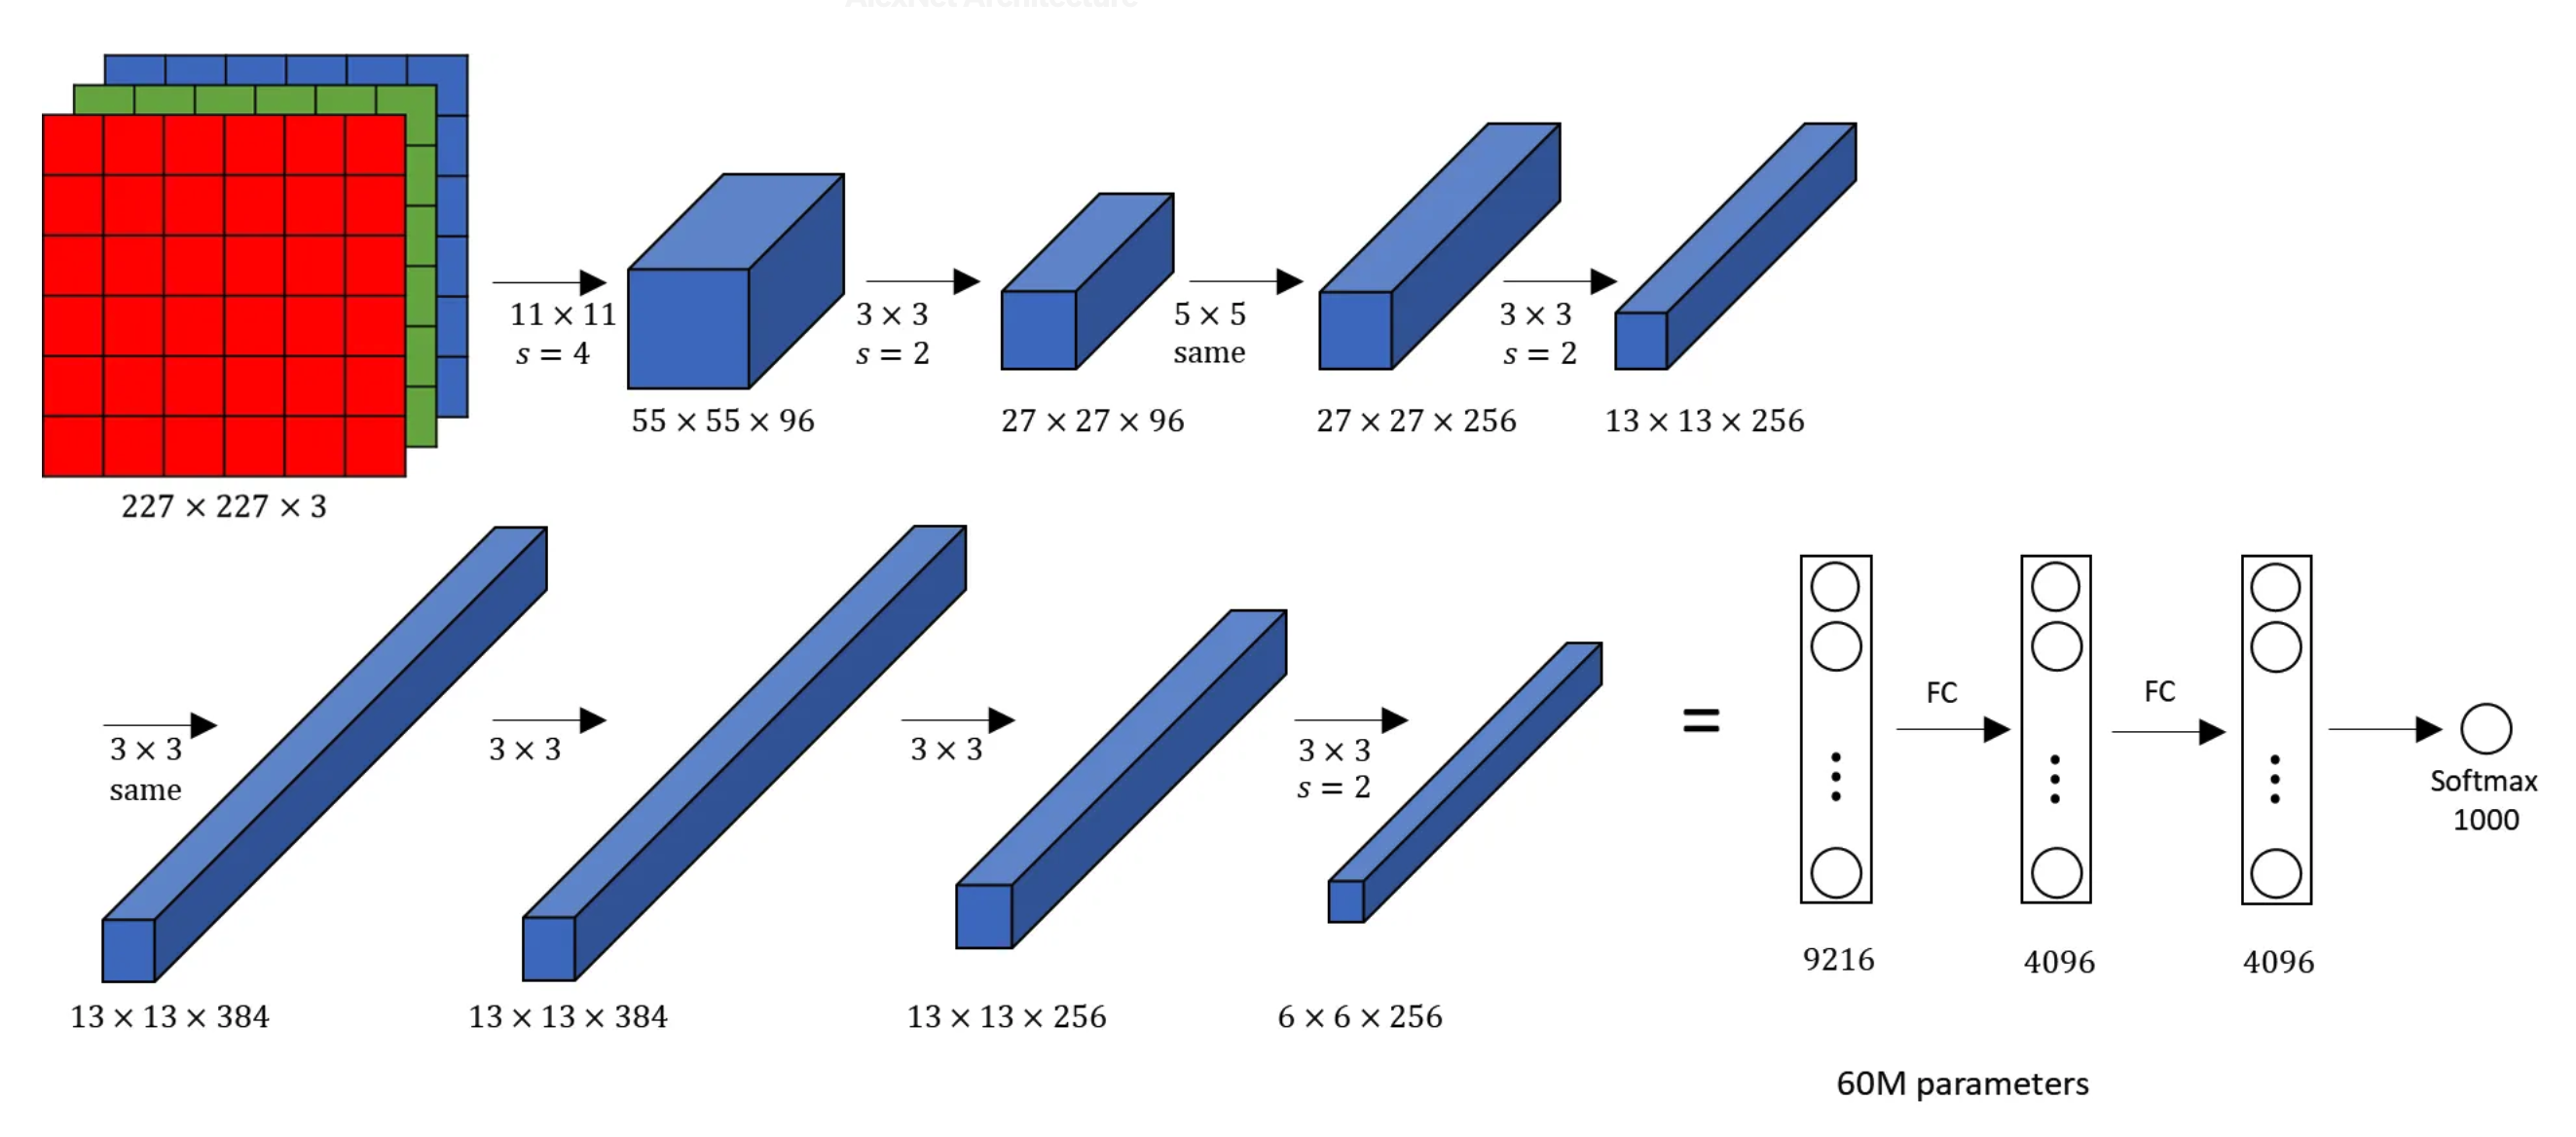
\includegraphics[width=15cm]{alexnet}
\end{center}

{\footnotesize Krizhevsky, Sutskever \& Hinton (2012, NeurIPS) --- 15.3\% top-5 error vs.\ 26.2\% for non-DL. Launched the DL agenda Lec.\ 4 turns onto dynamic macro.}
\end{frame}

\begin{frame}{Input Convex Neural Networks (ICNNs)}
\begin{itemize}
\item \textbf{Motivation:} In economics, many functions are known to be convex or concave: cost functions, duality mappings, value functions (after sign change).

\medskip
\item \textbf{ICNN architecture} (Amos, Xu \& Kolter 2017, ICML): ensure $f(x;\theta)$ is convex in $x$ by construction:
\begin{align*}
\mathbf{z}^{(0)} &= x \\
\mathbf{z}^{(\ell+1)} &= \sigma\!\left(\underbrace{W^{(\ell)}}_{\geq 0} \mathbf{z}^{(\ell)} + A^{(\ell)} x + b^{(\ell)}\right), \quad \ell = 1,\ldots,L-1
\end{align*}

\item \textbf{Key constraints:}
\begin{itemize}
\item Weights $W^{(\ell)} \geq 0$ (element-wise non-negative) for $\ell \geq 1$
\item Activation $\sigma$ must be convex and non-decreasing (ReLU, softplus)
\item ``Pass-through'' connections $A^{(\ell)} x$ can have unconstrained weights
\end{itemize}

\medskip
\item \textbf{Result:} The composition of convex, non-decreasing functions with non-negative weights preserves convexity.

\medskip
\item \textbf{For concavity:} Use $g(x) = -f(x;\theta)$ where $f$ is an ICNN. \emph{Lec.\ 4 T4 revisits with macro-validation framing (Lab 3A/6B).}
\end{itemize}
\end{frame}

% FullCourse Pass B addition: induction proof for ICNN convexity.
\begin{frame}{ICNN: Proof Sketch (Why It's Convex)}
We prove by induction that each $z_l(x)$ is convex in $x$.

\vspace{0.2cm}
\textbf{Step 1: Base Case}
\begin{itemize}
  \item $z_0(x) = x$ is linear; any linear function is both convex and concave.
\end{itemize}

\vspace{0.2cm}
\textbf{Step 2: Inductive Step}
\[
  z_{l+1}(x) = \sigma\bigl(W_z^{(l)} z_l(x) + W_x^{(l)} x + b_l\bigr)
\]
\begin{itemize}
  \item By induction, $z_l(x)$ is convex.
  \item With $W_z^{(l)} \geq 0$: $W_z^{(l)} z_l(x)$ is a non-negative sum of convex functions $\Rightarrow$ convex.
  \item Adding linear term $W_x^{(l)} x + b_l$ preserves convexity.
  \item Applying convex, non-decreasing $\sigma(\cdot)$ to a convex argument preserves convexity.
\end{itemize}

\vspace{0.15cm}
\textbf{Therefore}: All layers $z_l(x)$, and hence $f(x)$, are convex in $x$. \emph{(Lec.\ 4 T4 uses this directly on the Bellman value function.)}
\end{frame}

% FullCourse Pass B addition: expressivity theorem.
\begin{frame}{Do Constraints Limit Expressivity?}
\textbf{The concern}: By restricting $W_z \geq 0$, do we lose the universal approximation property?

\vspace{0.3cm}
\textbf{Theorem} (Chen, Shi, \& Zhang, 2019):
\begin{quote}
An Input Convex Neural Network can approximate \emph{any} convex function over a compact domain to arbitrary accuracy.
\end{quote}
{\footnotesize Reference: Chen, Y., Shi, Y., \& Zhang, B.\ (2019). \emph{Optimal Control via Neural Networks: A Convex Approach}. International Conference on Learning Representations (ICLR).}

\vspace{0.2cm}
\textbf{Intuition}:
\begin{itemize}
  \item A maximum of affine functions ($\max_i\{a_i^\top x + b_i\}$) is convex and can approximate any convex shape.
  \item An ICNN with ReLU activations acts as a hierarchical max-affine approximator.
\end{itemize}

\vspace{0.2cm}
\textbf{Economist's take:} You impose a \textbf{shape restriction} (convexity) without imposing a specific parametric form (CES, Cobb-Douglas). Architecture encodes theory; data still choose the function inside the theory-consistent class. \emph{(Lec.\ 4 T4 deploys this in dynamic equilibrium.)}
\end{frame}

% FullCourse Pass B addition: Partial ICNN for V(k,z) with concave-in-k, free-in-z.
\begin{frame}{Partial ICNN (PICNN): The Macro Reality}
\textbf{The issue}: Value functions $V(k, z)$ are typically:
\begin{itemize}
  \item \textbf{Concave} in endogenous states $k$ (capital, assets)
  \item \textbf{Non-concave / arbitrary} in exogenous states $z$ (TFP, income shocks)
\end{itemize}
A standard ICNN would incorrectly enforce convexity on $z$ as well.

\vspace{0.3cm}
\textbf{Solution}: Partial ICNN (PICNN, Amos et al.\ 2017) --- two paths combined so that convexity holds in $k$ for every fixed $z$:
\begin{enumerate}
  \item \textbf{Free path for $z$:} $u_l = \tanh(\widetilde W^{(l)}_u u_{l-1} + \widetilde b^{(l)}_u)$ (unconstrained FFNN of $z$).
  \item \textbf{Convex path for $k$, gated by $z$:}
  \[
    z_{l+1} = \sigma\Bigl(\underbrace{W^{(l)}_z\,(z_l \odot u_l)}_{W^{(l)}_z\geq 0} + W^{(l)}_x\,k + b^{(l)}\Bigr)
  \]
  where $\odot$ is element-wise multiplication; $u_l$ acts as a $z$-dependent positive gate on $z_l$.
\end{enumerate}

\textbf{Convexity in $k$}: at fixed $z$, $u_l$ is constant. Non-negative scaling, adding linear-in-$k$, and applying convex non-decreasing $\sigma$ all preserve convexity.
\end{frame}

% FullCourse Pass B addition: optimization landscape comparison.
\begin{frame}{Landscape Geometry: Why FFNNs Get Stuck}
\begin{columns}
  \begin{column}{0.4\textwidth}
    \textbf{Standard FFNN loss surface:}
    \begin{itemize}
      \item Rugged, non-convex.
      \item Many local minima.
      \item Outcome depends on initialization.
    \end{itemize}

    \vspace{0.3cm}
    \emph{Implication:} Re-train the same model with a different seed, get a different fit. Hard to audit; hard to publish.
  \end{column}

  \begin{column}{0.6\textwidth}
    \centering
    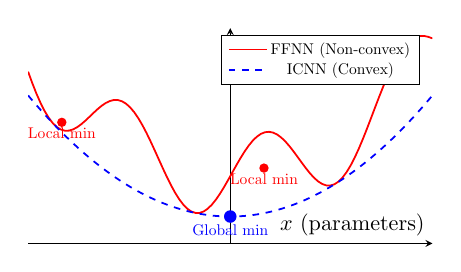
\begin{tikzpicture}[scale=0.8]
      \begin{axis}[
        width=8cm, height=5cm,
        axis lines=center,
        xlabel=$x$ (parameters), ylabel=Loss,
        xtick=\empty, ytick=\empty,
        ymin=0, ymax=8, xmin=-3, xmax=3,
        legend pos=north east,
        legend style={nodes={scale=0.7, transform shape}}
      ]
        \addplot[red, thick, domain=-3:3, samples=100]
          {0.5*x^2 + 1.5*sin(deg(3*x)) + 2.5};
        \addlegendentry{FFNN (Non-convex)}

        \addplot[blue, thick, dashed, domain=-3:3, samples=100]
          {0.5*x^2 + 1};
        \addlegendentry{ICNN (Convex)}

        \node[circle,fill=red,inner sep=1.5pt] at (axis cs:-2.5, 4.5) {};
        \node[red, below, scale=0.7] at (axis cs:-2.5, 4.5) {Local min};
        \node[circle,fill=red,inner sep=1.5pt] at (axis cs:0.5, 2.8) {};
        \node[red, below, scale=0.7] at (axis cs:0.5, 2.8) {Local min};

        \node[circle,fill=blue,inner sep=2pt] at (axis cs:0, 1) {};
        \node[blue, below, scale=0.7] at (axis cs:0, 0.9) {Global min};
      \end{axis}
    \end{tikzpicture}
  \end{column}
\end{columns}
\end{frame}

\begin{frame}{Why Convexity Matters for Macro Solvers}
\begin{itemize}
\item \textbf{Bellman / Euler equations have a unique fixed point} (under standard contraction conditions). A solver that converges to a \emph{local} minimum of the residual is not converging to that fixed point.

\medskip
\item \textbf{Reproducibility:} For a published paper, the policy function should not depend on the random seed. Convex training removes that dependence.

\medskip
\item \textbf{HA models compound the problem:} Aiyagari and Krusell--Smith require thousands of inner solves at every outer iteration. A 5\% chance of a bad local min per inner solve becomes a near-certain failure mode at scale.

\medskip
\item \textbf{Validation cost:} Without convexity guarantees, every solution needs a hand-checked sanity audit (analytical limit, Euler residual heatmap --- Lec.\ 4 T3). With convexity, validation is once at the architecture level.
\end{itemize}
\end{frame}

\begin{frame}{The ICNN Advantage: Bounding Optimization Risk}
\begin{itemize}
\item \textbf{Restated formally:} An ICNN makes $f(x;\theta)$ convex in its \emph{input} $x$ by construction, so \emph{inference} (optimizing/inverting over $x$ at fixed $\theta$) is a convex problem with a unique global optimum. Training over the parameters $\theta$ remains non-convex (cf.\ T3's non-convex loss landscape); convexity is a property of the learned function, not of the loss surface. For the convex inference subproblem, gradient descent's worst case is $O(1/T)$ convergence (Nesterov 2018, \emph{Lectures on Convex Optimization}).

\medskip
\item \textbf{Reference theorem:} Chen, Shi \& Zhang (2019), ICLR, ``Optimal Control via Neural Networks: A Convex Approach'' --- shows that the ICNN-parameterized optimal control problem has the same convex structure as the underlying linear-quadratic regulator.

\medskip
\item \textbf{Macro corollary:} You can swap a hand-coded convex solver (Sirignano \& Spiliopoulos 2018 (DGM), Maliar et al.\ 2021 deep-learning Euler method) for an ICNN-based solver without losing convergence guarantees. The architecture provides the math; PyTorch provides the speed.

\medskip
\item \textbf{Cost:} Restricted expressivity (Lec.\ 3 T4 ``Do Constraints Limit Expressivity?''). Partial ICNN (Amos et al.\ 2017) recovers most of it.
\end{itemize}
\end{frame}

% FullCourse Pass B addition: ICNN PyTorch reference implementation.
\begin{frame}[fragile]{ICNN: Robust PyTorch Implementation}
\textbf{Strategy}: Use reparameterization (Softplus) instead of clamping to enforce $W_z \geq 0$.
\vspace{-0.2cm}
\begin{lstlisting}[style=pythonstyle,basicstyle=\ttfamily\tiny]
class ICNN(nn.Module):
    def __init__(self, d_in, hidden_sizes):
        super().__init__()
        # Passthrough weights (Input -> Hidden) [unconstrained]
        self.W_x = nn.ParameterList([
            nn.Parameter(torch.randn(h, d_in))
            for h in hidden_sizes])
        # Recurrent weights (Hidden -> Hidden) [unconstrained params]
        # Apply Softplus() during forward pass to enforce W_z >= 0
        self.W_z_params = nn.ParameterList([
            nn.Parameter(torch.randn(h, h_prev))
            for h, h_prev in zip(hidden_sizes[1:], hidden_sizes[:-1])])
        self.biases = nn.ParameterList([
            nn.Parameter(torch.zeros(h)) for h in hidden_sizes])

    def forward(self, x):
        z = x
        for i, (Wz_p, Wx, b) in enumerate(
                zip(self.W_z_params, self.W_x, self.biases)):
            Wz = F.softplus(Wz_p)  # Enforce non-negativity
            z_next = F.linear(z, Wz) + F.linear(x, Wx) + b
            z = F.relu(z_next)
        return z
\end{lstlisting}
\end{frame}

\begin{frame}{Monotone Neural Networks}
\begin{itemize}
\item \textbf{Motivation:} Economic theory often implies monotonicity:
\begin{itemize}
\item Demand is non-increasing in price (law of demand)
\item Consumption is non-decreasing in wealth (normal goods)
\item Value functions are non-decreasing in the state
\end{itemize}

\medskip
\item \textbf{Architecture for monotonicity in input $x_j$:}
\begin{itemize}
\item Constrain all weights connecting from $x_j$ through the network to be \textbf{non-negative}
\item Use \textbf{non-decreasing} activation functions (ReLU, sigmoid, softplus)
\item Composition of non-decreasing functions is non-decreasing
\end{itemize}

\medskip
\item \textbf{Partial monotonicity:} Can enforce monotonicity w.r.t.\ \emph{some} inputs while leaving others unconstrained --- matching economic theory that demand is monotone in price but non-monotone in income (Giffen goods aside).

\medskip
\item \textbf{Practical enforcement:} After each gradient step, project weights to $\mathbb{R}_+$ via $w \leftarrow \max(w, 0)$ or use $w = \exp(\tilde{w})$ reparameterization.
\end{itemize}
\end{frame}

% FullCourse Pass B addition: monotone NN architecture diagram.
\begin{frame}{Monotone NN: Architecture --- Partial Monotonicity}
\begin{columns}
  \begin{column}{0.5\textwidth}
    \textbf{Objective}: Ensure $f(x)$ is non-decreasing in selected inputs:
    \[
      x_i \uparrow \;\Rightarrow\; f(x) \uparrow
    \]

    \vspace{0.2cm}
    \textbf{Two necessary constraints}:
    \begin{enumerate}
      \item \textbf{Non-negative weights}: $W^{(l)} \geq 0$ for monotone-input paths (biases unconstrained).
      \item \textbf{Monotonic activations}: $\sigma'(\cdot) \geq 0$ (ReLU, Sigmoid, Tanh, Softplus).
    \end{enumerate}

    \vspace{0.2cm}
    \textbf{Partial monotonicity:} Some inputs monotone (e.g., income $\to$ consumption); others free (e.g., interest rate $\to$ savings). Mirror the partial-ICNN trick.
  \end{column}

  \begin{column}{0.5\textwidth}
    \centering
    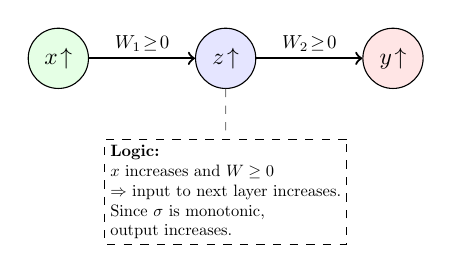
\begin{tikzpicture}[scale=0.85, transform shape,
      neuron/.style={circle, draw, minimum size=0.9cm},
      arrow/.style={->, thick}
    ]
      \node[neuron, fill=green!10] (I) at (0,0) {$x\!\uparrow$};
      \node[neuron, fill=blue!10] (H) at (2.5,0) {$z\!\uparrow$};
      \node[neuron, fill=red!10] (O) at (5,0) {$y\!\uparrow$};

      \draw[arrow] (I) -- (H) node[midway, above, scale=0.8] {$W_1 \!\geq\! 0$};
      \draw[arrow] (H) -- (O) node[midway, above, scale=0.8] {$W_2 \!\geq\! 0$};

      \node[draw, dashed, align=left, scale=0.7] at (2.5, -2) {
        \textbf{Logic:} \\
        $x$ increases and $W \geq 0$\\
        $\Rightarrow$ input to next layer increases.\\
        Since $\sigma$ is monotonic,\\
        output increases.
      };
      \draw[dashed, gray] (H) -- (2.5, -1.1);
    \end{tikzpicture}
  \end{column}
\end{columns}
\end{frame}

\begin{frame}{Monotone NN: Enforcement and Economic Examples}
\begin{itemize}
\item \textbf{Enforcement (same two methods as ICNN):}
\begin{itemize}
\item \emph{Clamping:} $W \leftarrow \max(W, 0)$ after each gradient step. Simple but can kill neurons (dead-ReLU analogue).
\item \emph{Reparameterization (Softplus):} train an unconstrained $\widetilde W$ and use $W = \mathrm{softplus}(\widetilde W) = \log(1+e^{\widetilde W})$. Preferred --- gradients flow.
\end{itemize}

\medskip
\item \textbf{Where macro needs monotonicity:}
\begin{itemize}
\item \emph{Wage curves} $w(\text{skill})$ --- weakly increasing.
\item \emph{Consumption functions} $c(\text{wealth})$ --- non-decreasing in wealth.
\item \emph{Demand curves} $q(p)$ --- non-increasing in price (flip sign).
\item \emph{Value functions} $V(k)$ in growth models --- monotone in capital.
\end{itemize}

\medskip
\item \textbf{PyTorch idiom:} wrap each linear layer's weight as \texttt{F.softplus(W\_raw)} in the forward call; train normally with AdamW. No special optimizer needed.
\end{itemize}
\end{frame}

\begin{frame}{Economic Applications of Constrained Architectures}
\begin{itemize}
\item \textbf{ICNN for optimal transport / Wasserstein distance:}
\begin{itemize}
\item Kantorovich duality: $W_1(\mu,\nu) = \sup_{f \text{ 1-Lipschitz}} \mathbb{E}_\mu[f] - \mathbb{E}_\nu[f]$
\item ICNNs parameterize the convex conjugate --- used in generative models and distributional analysis
\end{itemize}

\medskip
\item \textbf{Concave value functions:}
\begin{itemize}
\item In many macro models, $V(k)$ is concave in capital
\item Approximate $V$ with $-\text{ICNN}(k)$ to enforce concavity \emph{by construction}
\item Eliminates spurious non-concavities from unconstrained approximation
\end{itemize}

\medskip
\item \textbf{Monotone policy functions:}
\begin{itemize}
\item Savings policy $a'(a,z)$ is typically increasing in current assets $a$
\item Monotone networks guarantee this without post-hoc corrections
\end{itemize}

\medskip
\item \textbf{General principle:} Encoding economic structure into the network architecture reduces the hypothesis space, improves sample efficiency, and produces economically interpretable solutions.
\end{itemize}
\end{frame}

% FullCourse Pass B addition: Shephard's-lemma worked example.
\begin{frame}{Worked Example: Recovering Preferences via ICNN}
\textbf{Economic problem: Expenditure minimization}
\begin{align*}
  E(p, u) &= \min_{c \geq 0}\; p \cdot c \\
  \text{s.t.}\quad & U_\theta(c) \geq u \quad \text{(target utility)}
\end{align*}

\textbf{The ``structured'' solution}:
\begin{itemize}
  \item Learn the expenditure function $E_\theta(p, u)$ using a Concave ICNN.
  \item \textbf{Theory}: $E(p, u)$ must be concave in prices $p$ --- a structural property of the expenditure function.
\end{itemize}

\textbf{Why this is powerful}:
\begin{enumerate}
  \item \textbf{Shephard's Lemma + Auto-Diff}: $c^*(p, u) = \nabla_p E_\theta(p, u)$ --- demand functions for free.
  \item \textbf{Integrability}: Because $E_\theta$ is structurally concave, the resulting demands satisfy Slutsky-matrix properties by construction.
\end{enumerate}

\emph{Same recipe in Lec.\ 4 T4 with $V(k,z)$ as the macroeconomist's first ICNN.}
\end{frame}

% FullCourse Pass B addition: architecture cheat-sheet for picking constrained nets.
\begin{frame}{Choosing the Right Architecture: Cheat-Sheet}
\textit{Don't use a black box when you have a blueprint.}

\vspace{0.15cm}
\centering
\renewcommand{\arraystretch}{1.2}
\scriptsize
\begin{tabular}{p{0.16\textwidth}p{0.22\textwidth}p{0.32\textwidth}p{0.18\textwidth}}
\toprule
\textbf{Architecture} & \textbf{Shape constraint} & \textbf{Where useful in macro} & \textbf{Reuse} \\
\midrule
FFNN (baseline) & None & Generic regression, forecasting, classification & Lec 3 lab \\
CNN / AlexNet & Translation invariance & Satellite imagery, spatial data; not core macro & --- \\
\rowcolor{blue!5} ICNN & Input convexity & Bellman equation surfaces, cost \& value functions & Lec.\ 4 T4, Lab 3A/6B \\
\rowcolor{blue!5} PICNN & Partial convexity in $k$ & Aiyagari, growth model with shocks $z$ & Lec.\ 4 T4 \\
\rowcolor{blue!5} Monotone NN & Partial monotonicity & Wage curves, consumption rules, demand & Lec.\ 4 T4 \\
DEQ & Implicit fixed point & Equilibrium-as-layer; HA models & Lec.\ 6 \\
Dropout (regularizer) & --- & Overfitting control & all labs \\
\bottomrule
\end{tabular}

\vspace{0.15cm}
\raggedright\footnotesize
\textbf{Takeaway}: Structured architectures (shaded) encode economic theory directly --- you trade some flexibility for guarantees that match the problem.
\end{frame}

%=============================================================================
\section{Case Study: Curve Fitting and PyTorch}

\sectiondivider{Case Study: Curve Fitting and PyTorch}{One function, three approximators --- and your first PyTorch training loop}

\begin{frame}{Case Study: DNN vs.\ Polynomial vs.\ Chebyshev}
\begin{itemize}
\item \textbf{Objective:} Approximate a ``kinked'' function using three methods:
\begin{itemize}
    \item Deep Neural Network (DNN)
    \item Traditional polynomial approximation (\texttt{np.polyfit})
    \item Chebyshev polynomial approximation
\end{itemize}

\medskip
\item \textbf{Why this matters for economists:}
\begin{itemize}
    \item Many economic models feature kinks: borrowing constraints, tax brackets, occasionally binding constraints
    \item Polynomials suffer from \textbf{Gibbs phenomenon} near discontinuities
    \item DNNs with ReLU activations handle kinks naturally (piecewise linear)
\end{itemize}

\medskip
\item \textbf{Test function:}
\[
y(x) = \begin{cases} \alpha\beta\, x^\alpha & x \leq 0.5 \\ 2\alpha\beta\, x^\alpha & x > 0.5 \end{cases}
\]
A power function with a discrete jump at $x=0.5$ --- like a policy threshold.
\end{itemize}
\end{frame}

\begin{frame}{Example: GDP Forecasting with a Tiny MLP}
\begin{columns}[T]
\begin{column}{0.50\textwidth}
\footnotesize
\begin{itemize}
\item \textbf{Objective:} Predict next-quarter real GDP growth $g_t$ from four lags.

\item \textbf{Input:} $\mathbf{x}_t = (g_{t-1}, g_{t-2}, g_{t-3}, g_{t-4})$

\item \textbf{Architecture:} 4 $\to$ 16 (ReLU) $\to$ 8 (ReLU) $\to$ 1 (Linear).

\item \textbf{Why a NN?} GDP dynamics are state-dependent: shocks persist differently in recessions vs.\ expansions; AR models miss this.

\item \textbf{Loss:} MSE.
\end{itemize}
\end{column}

\begin{column}{0.50\textwidth}
\centering
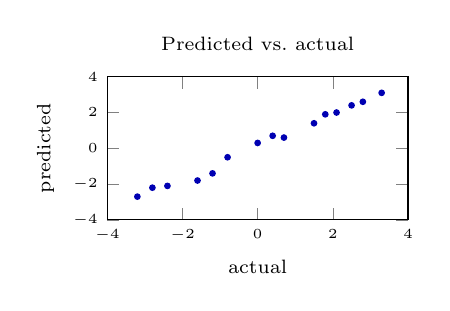
\begin{tikzpicture}
\begin{axis}[
    width=5.4cm, height=3.4cm,
    title={\scriptsize Predicted vs.\ actual},
    xlabel={\scriptsize actual}, ylabel={\scriptsize predicted},
    xmin=-4, xmax=4, ymin=-4, ymax=4,
    tick label style={font=\tiny}, label style={font=\tiny}, title style={font=\scriptsize},
    only marks, mark size=1pt,
]
\addplot[blue!70!black, mark=*] coordinates {
(-3.2,-2.7) (-2.4,-2.1) (-1.6,-1.8) (-0.8,-0.5) (0.0,0.3) (0.7,0.6) (1.5,1.4) (2.1,2.0) (2.8,2.6) (3.3,3.1) (-2.8,-2.2) (-1.2,-1.4) (0.4,0.7) (1.8,1.9) (2.5,2.4)
};
\addplot[red, thick, dashed, domain=-4:4] {x};
\end{axis}
\end{tikzpicture}

\vspace{1mm}
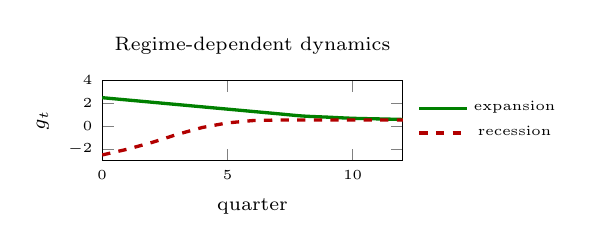
\begin{tikzpicture}
\begin{axis}[
    width=5.4cm, height=2.6cm,
    title={\scriptsize Regime-dependent dynamics},
    xlabel={\scriptsize quarter}, ylabel={\scriptsize $g_t$},
    xmin=0, xmax=12, ymin=-3, ymax=4,
    tick label style={font=\tiny}, label style={font=\tiny}, title style={font=\scriptsize},
    legend style={font=\tiny, draw=none, at={(1.02,0.5)}, anchor=west, fill=none},
]
\addplot[green!50!black, very thick, smooth] coordinates {
(0,2.5) (1,2.3) (2,2.1) (3,1.9) (4,1.7) (5,1.5) (6,1.3) (7,1.1) (8,0.9) (9,0.8) (10,0.7) (11,0.65) (12,0.6)
};
\addlegendentry{expansion}
\addplot[red!70!black, very thick, dashed] coordinates {
(0,-2.5) (1,-2.0) (2,-1.4) (3,-0.7) (4,-0.1) (5,0.3) (6,0.5) (7,0.55) (8,0.55) (9,0.55) (10,0.55) (11,0.55) (12,0.55)
};
\addlegendentry{recession}
\end{axis}
\end{tikzpicture}
\end{column}
\end{columns}
\end{frame}

\begin{frame}[fragile]{PyTorch: Defining and Training the Model}

\begin{lstlisting}[style=pythonstyle]
import torch
import torch.nn as nn
import torch.optim as optim

class GDPNet(nn.Module):
    def __init__(self):
        super().__init__()
        self.net = nn.Sequential(
            nn.Linear(4, 16), nn.ReLU(),
            nn.Linear(16, 8), nn.ReLU(),
            nn.Linear(8, 1)
        )
    def forward(self, x):
        return self.net(x)

model = GDPNet()
criterion = nn.MSELoss()
optimizer = optim.Adam(model.parameters(), lr=0.001)

for epoch in range(1000):
    optimizer.zero_grad()          # 1. Reset gradients
    y_hat = model(X_batch)         # 2. Forward pass
    loss = criterion(y_hat, y_batch) # 3. Compute loss
    loss.backward()                # 4. Backpropagation
    optimizer.step()               # 5. Update weights
\end{lstlisting}
\end{frame}

\begin{frame}[fragile]{PyTorch: Class-Based Network with Batch Normalization}

\begin{lstlisting}[style=pythonstyle]
class KinkNet(nn.Module):
    """Network for approximating kinked functions."""
    def __init__(self, input_dim, hidden_dim1,
                 hidden_dim2, output_dim=1):
        super().__init__()
        self.net = nn.Sequential(
            nn.Linear(input_dim, hidden_dim1),
            nn.BatchNorm1d(hidden_dim1),
            nn.ReLU(),
            nn.Linear(hidden_dim1, hidden_dim2),
            nn.BatchNorm1d(hidden_dim2),
            nn.ReLU(),
            nn.Linear(hidden_dim2, output_dim)
        )

    def forward(self, x):
        return self.net(x)
\end{lstlisting}

\medskip
\textbf{Key additions:} \texttt{BatchNorm1d} normalizes activations within each mini-batch --- stabilizes training and acts as light regularization.
\end{frame}

%=============================================================================
\section{Lab Preview}

\sectiondivider{Lab Preview}{Hands-on: ML basics and the FOMC-minutes yield-curve application}

\begin{frame}{Lab: Machine Learning Basics and Applications}
\textbf{Notebook:} \texttt{Lec03\_Lab\_ML\_Basics.ipynb} --- one self-contained notebook, three parts.

\begin{tcolorbox}[colback=green!3, colframe=green!40, title=Part 1: Neural nets as flexible regression]
\begin{itemize}
\item Train a small PyTorch MLP to learn a consumption function $c=f(w)$ from noisy data --- ``a neural network is just non-parametric regression.''
\item \textbf{Universal approximation, hands-on:} build $\hat f(x)=a_0+\sum_i a_i\,\mathrm{ReLU}(w_i x+b_i)$ and watch ReLU units sum to $\sin x$; then see \textbf{implicit regularization} --- gradient descent finds the minimum-norm, smooth fit.
\end{itemize}
\end{tcolorbox}

\begin{tcolorbox}[colback=blue!3, colframe=blue!40, title=Parts 2--3: Two economic applications]
\begin{itemize}
\item \textbf{Predict the 10-year Treasury yield} from the policy rate + unemployment (live FRED data, synthetic fallback), using a proper \emph{time-series} split.
\item \textbf{Read the Fed's words:} turn hawkish/dovish sentences into bag-of-words features, classify with logistic regression, then a PyTorch MLP.
\end{itemize}
\end{tcolorbox}
\end{frame}

\begin{frame}{Lecture 3, Complete: One Map, Four Acts}
\textbf{The toolkit is assembled: you know why ML matters for economists, what a network is, how it trains, and how to bend it to economic theory.}

\LecThreeMap{0}

\vspace{0.05cm}
\footnotesize\textit{Every later lecture draws on this map: Lec.\ 4 turns these networks into Bellman/Euler solvers, Lec.\ 6 scales them to heterogeneous agents, and Lec.\ 7's transformers are the same approximation theory wearing attention.}
\end{frame}

\begin{frame}{Preview: What Lec.\ 4 Does With These Tools}
\begin{itemize}
\item \textbf{Lec.\ 4 T1 --- Motivation + optimal growth setup:} why grids fail in $d \geq 5$; AlphaGo-style intuition for macro state spaces.

\medskip
\item \textbf{Lec.\ 4 T2 --- Deep VFI + actor-critic preview:} the NN architectures of T2 + T4 deployed as Bellman solvers; actor-critic algorithm previewed for Lec.\ 5.

\medskip
\item \textbf{Lec.\ 4 T3 --- Euler equation as supervised learning:} the backprop machinery of T3 turned on first-order conditions; PyTorch implementation.

\medskip
\item \textbf{Lec.\ 4 T4 --- Structured NNs + validation:} ICNN + Monotone re-applied to dynamic macro with Lab 3A (ground-truth VFI) + Lab 3B (NN solution) + Euler-residual heatmap as the validation gate.
\end{itemize}

\medskip
\begin{center}
\footnotesize\textit{Lec.\ 5 then formalizes the RL machinery; Lec.\ 6 scales to heterogeneous-agent models.}
\end{center}
\end{frame}

\begin{frame}{Summary}
\begin{enumerate}
\item \textbf{Why ML:} Unstructured data, high-dimensional models, and non-linear dynamics make ML essential for modern macro research.

\medskip
\item \textbf{Neural Networks:} Universal approximators that compose linear transformations with nonlinear activations. Barron (1993): break the curse of dimensionality.

\medskip
\item \textbf{Training:} Forward pass $\to$ loss $\to$ backpropagation $\to$ gradient descent. Mini-batch SGD with Adam is the practical standard.

\medskip
\item \textbf{Regularization:} Weight decay, dropout, early stopping, batch normalization prevent overfitting --- the ML analogue of avoiding data mining.

\medskip
\item \textbf{Constrained Architectures:} ICNNs enforce convexity; monotone networks enforce monotonicity. Encoding economic structure into network design improves both accuracy and interpretability.

\medskip
\item \textbf{Next:} Lec.\ 4 applies these tools to \emph{solve} macro models --- deep learning meets the Bellman equation.
\end{enumerate}
\end{frame}

\end{document}
